\section{Delve into LLM Inference and Deployment}
\label{sec:challenges}

% Imagine a situation where your friend Alice wants to use a LLM on her personal computer to improve her novel-writing process. She needs to make a decision on which computer to purchase. How can Alice make an informed choice?
% Now, let's consider another scenario: Bob intends to use LLMs to offer legal document retrieval and Q\&A services for his colleagues at a small company. What factors should Bob take into consideration when making a decision in this case?

% In this section, we will introduce the LLMs inference and deployment. 
% By the end of this chapter, you will gain a clear understanding of the operational aspects of LLMs.
% and be equipped with insights to help Alice and Bob make informed decisions regarding their deployment.

\subsection{LLM Inference}
\label{sec:llm_inference}

% Nowadays, most large language models (LLMs) takes Transformer decoder architecture.
% It contains a embedding layer and a lot of sequential Transformer layers and a prediction head.
% The embedding layer xxx.
% Each Transformer layer contains a masked multi-head attention submodule (named MHA), a feedforward network (named MLP), and several layer normalization operations. Layers are put in sequence to make the model deeper.
% the output of the last Transformer layer is fed through one more linear layer to obtain the final output of the model (a classification, a next word/token etc.)

\begin{figure*}[t]
    \centering
    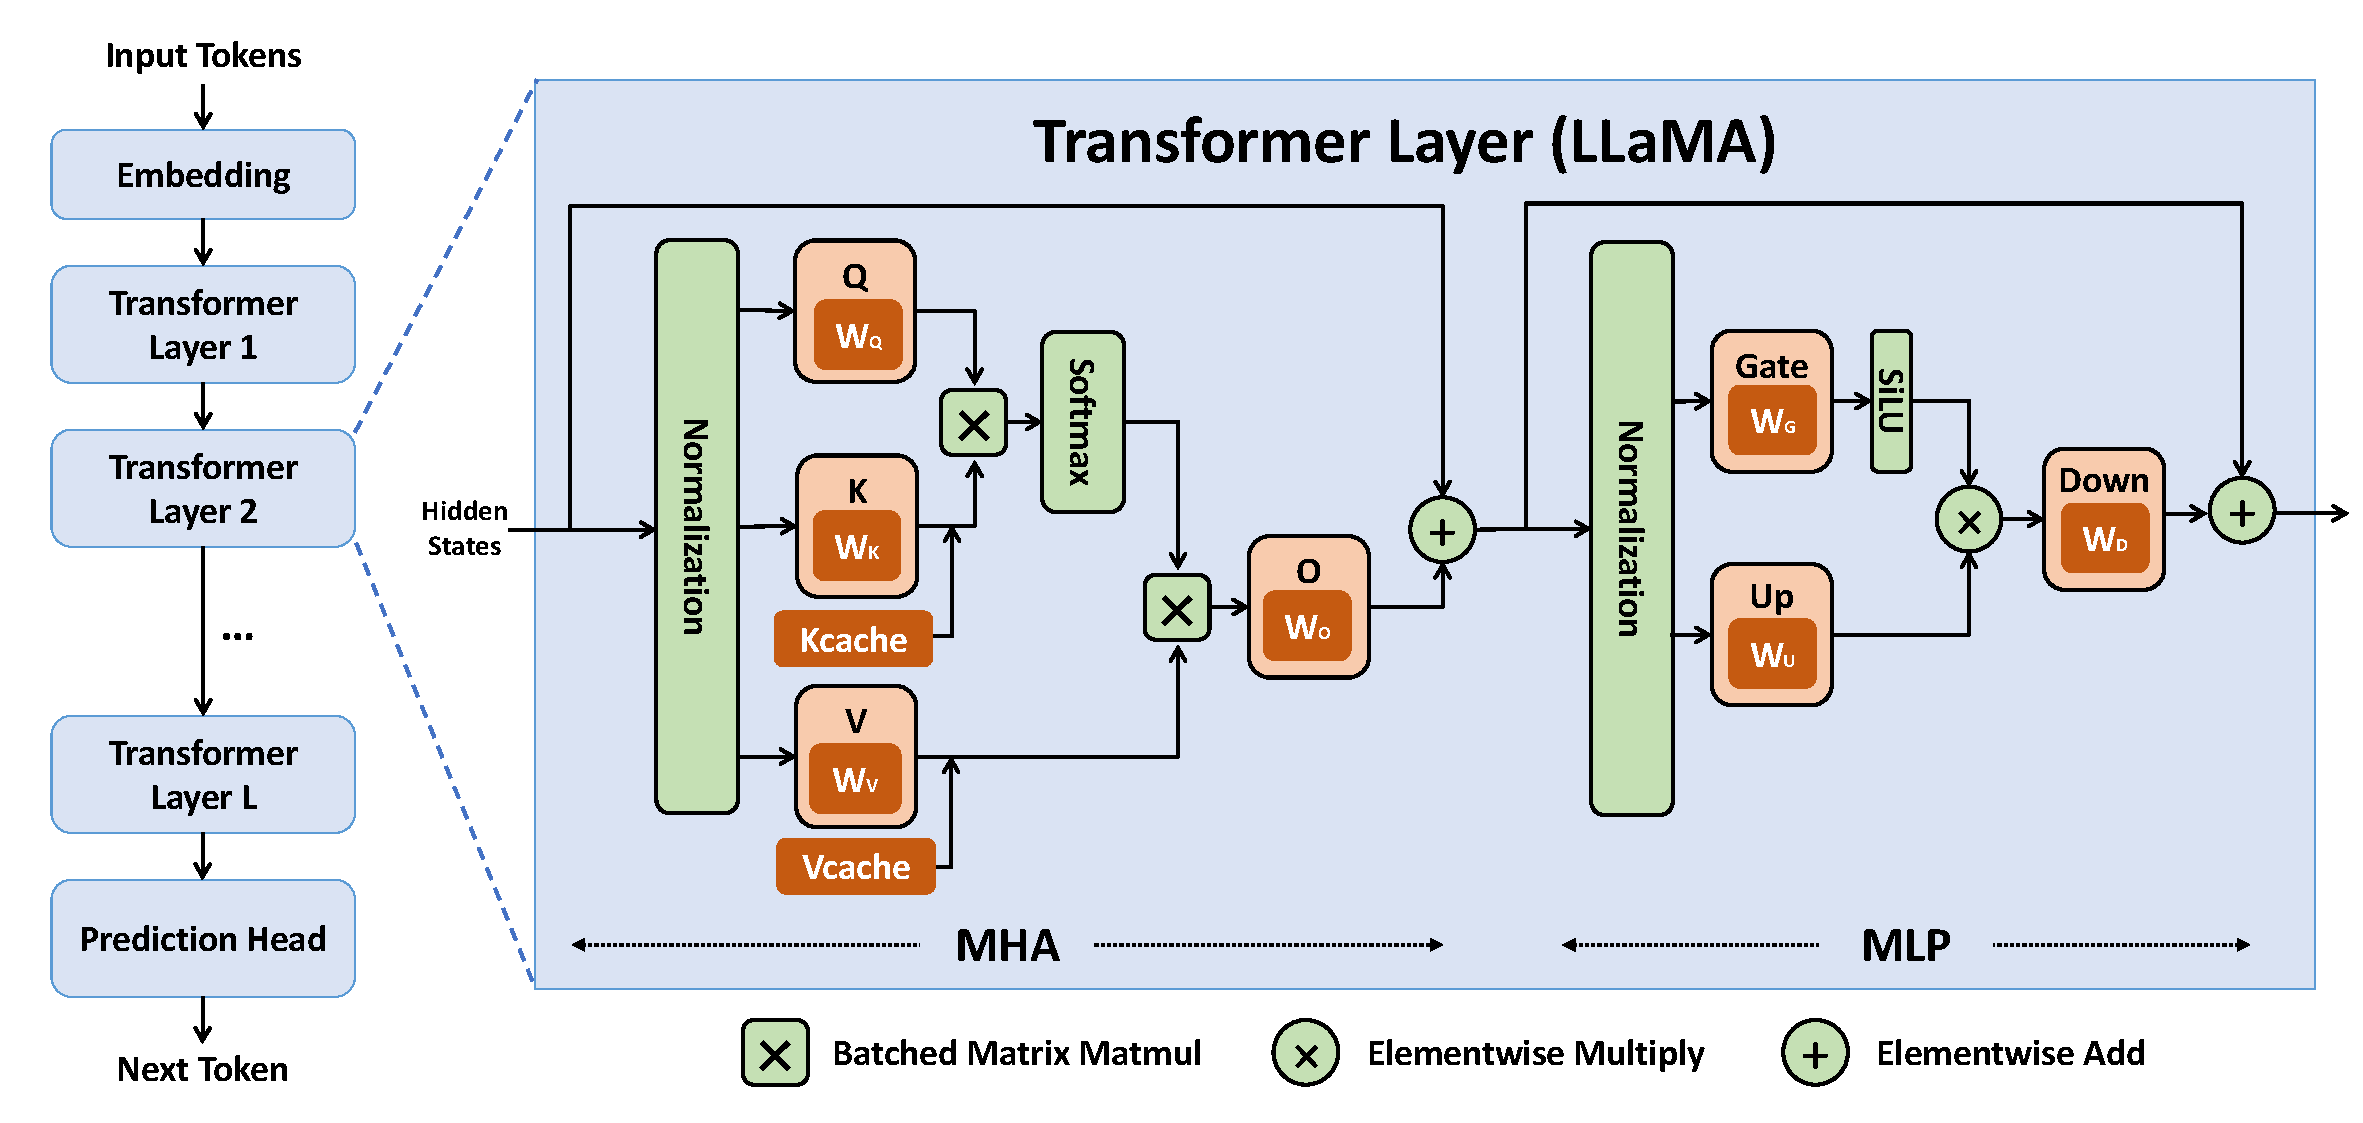
\includegraphics[width=0.8\linewidth]{ims/transformer_arch.pdf}
    % \vspace{-0.6in}
    \caption{Demonstration of the architecture of LLMs.}
    \label{fig:transformer_layer}
\end{figure*}

Nowadays, the prevailing architecture adopted by most large language models (LLMs) is the Transformer decoder architecture. 
Here we will provide a concise overview of its fundamental structure, with the option to refer to this survey~\cite{zhao2023survey} for a more in-depth understanding.
This structure comprises an embedding layer, a series of sequential Transformer layers, and a prediction head. Figure~\ref{fig:transformer_layer} demonstrated the architecture. 
% Let's delve into the intricacies of each component.

% This embedding module transform input token into a vector format. It undergoes a transformation of diverse input types, spanning from words to image patches, ultimately converting them into vector representations. This intricate process enhances the model's capability to process a wide array of sequential data. 
% The significance lies in the module's ability to map various input modalities into a uniform vector space, facilitating seamless processing in subsequent layers.

The embedding layer transform input tokens into the hidden states. 
The hidden states are sent to the Transformer layers.
Each Transformer layer consists of two components. 
Firstly, there is a masked multi-head attention module, denoted as \textbf{MHA}. 
% This module allows the model to focus on different parts of the input sequence, enhancing its capacity to capture dependencies and relationships within the data. 
Following MHA is a multi-layer perceptron submodule, labeled as \textbf{MLP}. 
% Additionally, layer normalization operations and residual connections are applied at the two submodules to maintain stability and aid in the model training process.
% The sequential arrangement of these Transformer layers aims to enhance the model's depth. 
The output from the last Transformer layer is then sent to the prediction head, which is responsible for predicting the next token after the input tokens.

Inference represents the process opposite to the training process. During training, a model learns from a vast dataset to capture the intricacies of language and context. The weights in model are updated. In contrast, during inference, a user inputs a \textbf{prompt}, and the LLM engages in a process of generating \textbf{responses}.
This process involves the model utilizing its fixed pre-trained weights to comprehend the input text and produce text as output. 
The inference process of Large Language Models (LLMs) is divided into two stages: the \textbf{Prefill Stage} and the \textbf{Decode Stage}.

% The inference of LLM is divided in two stages, \textbf{prefill} stage and \textbf{decode} stage.
% i) the prefill stage which takes a prompt sequence to generate the key-value cache (KV cache) for each transformer layer of the LLM; and ii) the decoding stage which utilizes and updates the KV cache to generate new tokens step-by-step, where the current token generation depends on previously generated tokens.

The Prefill Stage serves as the initial step in LLM inference. In this stage, the model takes a prompt sequence as input and engages in the generation of a key-value cache (KV cache) for each Transformer layer within the LLM. The KV cache plays a crucial role in storing and organizing information that the model deems relevant for subsequent token generation. Each Transformer layer is equipped with its own unique KV cache, and this prefilling process establishes the foundation for the subsequent decoding stage.

In the Prefill Stage, the Multi-Head Attention (MHA) creats key-value (KV) pairs that will be stored in the KV cache. Let's denote the input to a Transformer layer as $\mathbf{X}_{\text{pre}} \in \mathbb{R}^{n\times d}$, where $d$ is the hidden size and $n$ is the length of prompt token sequence. The layers in the MHA have weights represented by $\mathbf{W}_q$, $\mathbf{W}_k$, $\mathbf{W}_v$, and $\mathbf{W}_o$.
The query, key and value are computed through the following process:
\begin{align*}
\text{Query:} \quad \mathbf{Q}_{\text{pre}} &=  \mathbf{X}_{\text{pre}} \cdot \mathbf{W}_q \\
\text{Key:} \quad \mathbf{K}_{\text{pre}} &=  \mathbf{X}_{\text{pre}} \cdot \mathbf{W}_k \\
\text{Value:} \quad \mathbf{V}_{\text{pre}} &= \mathbf{X}_{\text{pre}} \cdot \mathbf{W}_v 
\end{align*}
The generated $\mathbf{K}_{\text{pre}}$ and $\mathbf{V}_{\text{pre}}$ are stored in the KV cache. The other computation in MHA can be formulated as~\footnote{We omit layer norm, position mask, and positional embedding for simplicity.}:
\begin{align*}
\mathbf{O}_{\text{pre}} &= \text{softmax}\left(\frac{\mathbf{Q}_{\text{pre}} \cdot \mathbf{K}_{\text{pre}}^T}{\sqrt{d}}\right) \cdot \mathbf{V}_{\text{pre}}\cdot \mathbf{W}_o +\mathbf{X}_{\text{pre}},
\end{align*}
where the output of MHA $\mathbf{O}_{\text{pre}} \in \mathbb{R}^{n\times d}$ is sent to the MLP.
The output of the MLP serves as the input for the next Transformer layer.


The Decode Stage represents the core of the LLM inference process. In the Decode Stage, the model uses the KV caches prepared earlier and might add new information to them. The goal here is to generate tokens, which are essentially words or parts of words. This happens step by step. The creation of each new token is influenced by the tokens that were generated before it, like building a sentence word by word.


In the Decode Stage, the MHA loads the previously stored KV cache $\mathbf{K}_{\text{cache}}$ and $\mathbf{V}_{\text{cache}}$. The input is $\mathbf{X}_{\text{dec}} \in \mathbb{R}^{1\times d}$. New key and value pairs are computed and concatenated to the existing cache:
\begin{align*}
\text{Query:} \quad \mathbf{Q}_{\text{dec}} &=  \mathbf{X}_{\text{dec}} \cdot \mathbf{W}_q \\
\text{Key:} \quad \mathbf{K}_{\text{cat}} &=  [\mathbf{K}_{\text{cache}}, \mathbf{X}_{\text{dec}} \cdot \mathbf{W}_k] \\
\text{Value:} \quad \mathbf{V}_{\text{cat}} &=  [\mathbf{V}_{\text{cache}}, \mathbf{X}_{\text{dec}} \cdot \mathbf{W}_v]
\end{align*}
These newly computed $\mathbf{X}_{\text{dec}} \cdot \mathbf{W}_k$ and $\mathbf{X}_{\text{dec}} \cdot \mathbf{W}_v$ are then appended to the KV cache. The other computation in MHA is carried out as follows:
\begin{align*}
\mathbf{O}_{\text{dec}} &= \text{softmax}\left(\frac{\mathbf{Q}_{\text{dec}} \cdot \mathbf{K}_{\text{cat}}^T}{\sqrt{d}}\right) \cdot \mathbf{V}_{\text{cat}} \cdot \mathbf{W}_o + \mathbf{X}_{\text{dec}}
\end{align*}
where the output of MHA $\mathbf{O}_{\text{dec}} \in \mathbb{R}^{1\times d}$ is sent to the MLP.
The output of the last Transformer layer is sent to the final prediction layer to predict the next token.

% \subsection{Considerations on Deployment}


% In the realm of large model inference and deployment, three key factors demand our attention: the computation capability of the hardware, the size of hardware memory, and the bandwidth of that memory. These elements intertwine, playing a pivotal role in the efficiency and success of deploying large models.

% Computation, memory footprint, and memory access are key considerations in the inference and deployment of large models. 
% For a given large model, we can calculate the theoretical computation, memory footprint, and memory access for both individual operations and the model as a whole.

% \textbf{Computation Capability}: The heart of the matter lies in the computation capability of the hardware. 
% First off, the hardware has to be able to handle the data flow for operations like matrix multiplication and non-linear functions (such as softmax). Also, it needs to support the data types used in these operations, like the common ones - FP16 and FP32, or even INT8 if the model is quantized. 
% If the hardware can handle all the operations needed by the LLMs, then there's a chance it can be deployed. And don't forget, the hardware needs enough computational power, meaning it should have plenty of processing units (such as CUDA cores in GPU). We can measure the computational capability by peak computational performance (operations per second, OPS).


% \textbf{Memory Size}: For LLMs, having sufficient memory is crucial to hold the weight of the model's parameters and intermediate results during inference. 
% LLMs' weights can be several gigabytes (GB) to even over a hundred GB for really big models.
% The KV cache changes based on how much text you're working with and the size of the group of tasks you're doing (batch size). 
% If you're dealing with a lot of text or have a big batch size, the KV cache can take up several GBs to tens of GBs of space. 


% \textbf{Memory Bandwidth}: Memory bandwidth refers to the rate at which data moves between the memory and the computation units.
% When data transfer is slow, the computation units have to wait idly for the data to arrive. This can pose a significant bottleneck for LLMs. In the next section, we will delve into a detailed explanation of this issue.


% Choosing the right hardware for LLMs isn't a one-size-fits-all situation because of the difference of various tasks. The differences in tasks mainly come down to batch size, the ratio between the prefill and decode stages, and the length of the sequences.
% % Take Alice, for example. She uses a single batch for her own needs and prefers long sequences for writing novels. Since her task is more focused on generating content, she needs a high ratio of the decode stage.
% % On the other hand, Bob needs multiple batches to cater to simultaneous queries from different people in the company. As his task is more about queries and retrieval, he requires a high ratio of the prefill stage.
% Next, we will take both the hardware and tasks into consideration and introduce how to evaluate the efficiency of inference.


\subsection{Roofline Model}
\label{sec:Rooflinemodel}

% 上面的介绍中已经详细介绍了两个大模型运行的流程，接下来我们就可以进入大模型部署的速度评估部分了，进而可以回答本section一开始Alice和Bob提出的问题。
% 要评估大型语言模型部署到特定的硬件上的运行速度有多快，需要同时考虑硬件特性和模型特性。
% 我们将会使用一种被广泛使用的技术——Roofline model来完成运行速度的评估。

% 我们知道，硬件设备运行一个算子，需要首先将数据从存储器（DDR或者HBM）中搬运到on-chip memory，然后片上的计算单元进行计算，最后将结果输出到存储器。
% 为了评估速度，需要同时考虑存储器的访存、以及计算单元的计算。
% The Roofline model 是一个很好的理论模型能够评估在特定硬件上部署一个模型的理论性能上限. 它能够显示模型中每个算子的运行是访存bottleneck还是计算bottleneck。
% 当一个操作要进行很多计算，而访存较少的时候，我们称这种情况为computation bottleneck。
% In such cases, the memory access units experience idle time.
% 详细说明xxxx

% Conversely, 当一个操作要进行很多访存，而计算较少的时候，我们称这种情况为memory bottleneck。 the computational units remain underutilized.
% 详细说明xxxx

Assessing the efficiency at which LLMs deploy onto specific hardware involves a comprehensive consideration of both hardware and model characteristics. To conduct this evaluation, we employ the Roofline model.
The Roofline model serves as an effective theoretical framework to assess the potential performance of deploying a model on particular hardware. 
% It provides insights into whether each operator within the model is constrained by memory access (referred to as a memory bottleneck) or computational capabilities (referred to as a computation bottleneck).

\begin{figure}[t]
    \centering
    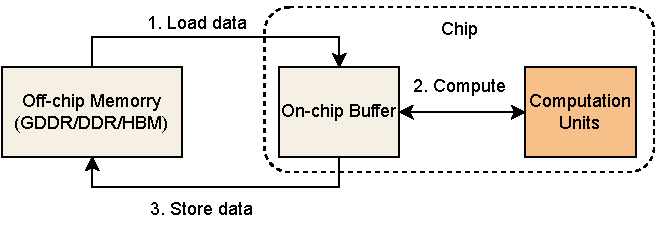
\includegraphics[width=0.95\linewidth]{ims/hardware_run.pdf}
    % \vspace{-0.6in}
    \caption{Execution of an operation on hardware.}
    \label{fig:hardware_run}
\end{figure}

As shown in Figure~\ref{fig:hardware_run}, the execution of a neural network layer on hardware devices entails the transfer of data from memory (DDR or HBM) to on-chip buffers, followed by computations performed by on-chip processing units, ultimately outputting results back to memory. 
Therefore, evaluating performance requires simultaneous consideration of memory access and processing unit capabilities.
If a layer involves extensive computations but minimal memory access, it is termed a computation bottleneck. 
This scenario leads to idle on the memory access. 
On the contrary, when a layer requires substantial memory access with fewer computational demands, it is referred to as a memory bottleneck. In this case, computational units remain underutilized. 
We can clearly distinguish between these two scenarios according to the Roofline model and provide performance upper bounds for different situations.

\begin{figure}[t]
    \centering
    \includegraphics[width=0.95\linewidth]{ims/Roofline_nvidia_A6000.pdf}
    % \vspace{-0.6in}
    \caption{Demonstration of the Roofline model of Nvidia A6000 GPU. The computation is in FP16.}
    \label{fig:Roofline}
\end{figure}

There are two steps to using the Roofline model:

1. \textbf{Plot the Roofline}: Determine the peak computational performance (operations per second, OPS) and peak memory bandwidth (bytes per second) specific to the target hardware device.\footnote{OPS refer to the number of operations per second. Each Multiply-Accumulate (MAC) operation counts two operations.}
Then create a graph with performance (OPS) on the y-axis and arithmetic intensity (OPs/byte) on the x-axis: Draw a horizontal line equal to the peak computational performance. This line represents the maximum achievable performance by the hardware device.
And draw a diagonal line from the origin with a slope equal to the peak memory bandwidth. This line represents the maximum memory bandwidth available
on the system, known as the memory Roofline.
Figure~\ref{fig:Roofline} demonstrates the Roofline model of Nvidia A6000 GPU.

2. \textbf{Analyze performance for layers}: Evaluate the performance of each layer in the model by quantifying both the number of operations (OPs) and the volume of data accessed from memory (bytes). Calculate the arithmetic intensity (OPs/byte) of each layer by dividing the required operations by the amount of data transferred. 
According to the graph created in the first step, the theoretical max performance for each layer is determined by the position on the graph corresponding to the x-axis value of arithmetic intensity. It allows us to ascertain whether the system is memory-bound or compute-bound at this point, guiding the determination of the subsequent optimization strategy.
% 回到第一步画的图上，这层理论的性能上限就是图中x为arithmetic intensity时Roofline线对应的位置。我们也能确定这个时候是memory-bound还是compute-bound，以此可以确定下一步的优化策略。


\begin{table}[tb]
\caption{Analysis for layers in Llama-2-7b using the Roofline model of Nvidia A6000 GPU. In this example, the sequence length is 2048 and the batch size is 1.} 
\label{tab:Llama_analysis} 
\resizebox{\linewidth}{!}{
\begin{tabular}{@{}cccccc@{}}
\toprule
Layer Name & OPs  & \begin{tabular}[c]{@{}c@{}}Memory\\ Access\end{tabular} & \begin{tabular}[c]{@{}c@{}}Arithmetic\\ Intensity\end{tabular} & \begin{tabular}[c]{@{}c@{}}Max\\ Performance\end{tabular} & Bound   \\ \midrule
\multicolumn{6}{c}{Prefill}                                                                                                                                                                                        \\ \midrule
q\_proj    & 69G  & 67M                                                     & 1024                                                           & 155T                                                      & compute \\
k\_proj    & 69G  & 67M                                                     & 1024                                                           & 155T                                                      & compute \\
v\_proj    & 69G  & 67M                                                     & 1024                                                           & 155T                                                      & compute \\
o\_proj    & 69G  & 67M                                                     & 1024                                                           & 155T                                                      & compute \\
gate\_proj & 185G & 152M                                                    & 1215                                                           & 155T                                                      & compute \\
up\_proj   & 185G & 152M                                                    & 1215                                                           & 155T                                                      & compute \\
down\_proj & 185G & 152M                                                    & 1215                                                           & 155T                                                      & compute \\
qk\_matmul & 34G  & 302M                                                    & 114                                                            & 87T                                                       & memory  \\
sv\_matmul & 34G  & 302M                                                    & 114                                                            & 87T                                                       & memory  \\
softmax    & 671M & 537M                                                    & 1.25                                                           & 960G                                                      & memory  \\
norm       & 59M  & 34M                                                     & 1.75                                                           & 1T                                                        & memory  \\
add        & 8M   & 34M                                                     & 0.25                                                           & 192G                                                      & memory  \\ \midrule
\multicolumn{6}{c}{Decode}                                                                                                                                                                                         \\ \midrule
q\_proj    & 34M  & 34M                                                     & 1                                                              & 768G                                                      & memory  \\
k\_proj    & 34M  & 34M                                                     & 1                                                              & 768G                                                      & memory  \\
v\_proj    & 34M  & 34M                                                     & 1                                                              & 768G                                                      & memory  \\
o\_proj    & 34M  & 34M                                                     & 1                                                              & 768G                                                      & memory  \\
gate\_proj & 90M  & 90M                                                     & 1                                                              & 768G                                                      & memory  \\
up\_proj   & 90M  & 90M                                                     & 1                                                              & 768G                                                      & memory  \\
down\_proj & 90M  & 90M                                                     & 1                                                              & 768G                                                      & memory  \\
qk\_matmul & 17M  & 17M                                                     & 0.99                                                           & 762G                                                      & memory  \\
sv\_matmul & 17M  & 17M                                                     & 0.99                                                           & 762G                                                      & memory  \\
softmax    & 328K & 262K                                                    & 1.25                                                           & 960G                                                      & memory  \\
norm       & 29K  & 16K                                                     & 1.75                                                           & 1T                                                        & memory  \\
add        & 4K   & 16K                                                     & 0.25                                                           & 192G                                                      & memory  \\ \bottomrule
\end{tabular}
}
\end{table}

There are two scenarios where resources are not fully utilized: When the model's computational intensity is below the turning point, residing in the red zone, it implies that the computational workload required per memory access is low. Even saturating the peak bandwidth does not fully utilize all computational resources. In such cases, the layer is constrained by memory access (memory-bound), and some computational units may remain idle.
If the layer is memory-bound, consider optimization techniques such as quantization, kernel fusion and increasing batch size to alleviate the memory footprint. 
Conversely, if the model's computational intensity is above the turning point, situated in the green zone, it suggests that the model requires only a small amount of memory access to consume a significant amount of computational capability. It implies that the layer is constrained by computation (compute-bound), with some memory units potentially remaining idle.
In this case, we should investigate strategies such as enabling low-bit computation to enhance computational efficiency. 
Detailed explanations of these methods will be provided in the subsequent sections.

% As an example, Table~\ref{tab:Llama_analysis} shows the analysis for layers in Llama-2-7b using the Roofline model of Nvidia A6000 GPU.
% 从表格中可以发现，在prefill stage大部分计算是compute-bound，因此能达到很高的performance。而decode stage中所有的计算都是memory-bound，并且performance远远低于这个GPU的计算单元所能提供的算力。
% 用户使用大模型的过程中，prefill stage只执行一次，而decode stage将会被反复执行以生成一段连续的输出结果。因此，针对decode阶段memory-bound的优化会是大模型推理优化的核心。

As an example, Table~\ref{tab:Llama_analysis} presents the analysis of layers in Llama-2-7b using the Roofline model on the Nvidia A6000 GPU.
From the table, we observe that during the prefill stage, the majority of computations are compute-bound, leading to high performance. 
Conversely, in the decode stage, all computations are memory-bound, resulting in performance significantly below the computational capacity of the GPU's computation units.
During the user's interaction with large models, the prefill stage executes only once, while the decode stage is repeatedly performed to generate a continuous output. Therefore, optimizing for the memory-bound characteristics of the decode stage becomes crucial for enhancing the inference performance of large models.


\subsection{LLM-Viewer}
\label{sec:llmviewer}

% Except considering operation-wise computation and memory access in the Roofline model, 
% LLM中存在很多Transformer layers，每层中存在多种operations。不同的LLM的operations还不一样。此外，我们还需要追踪memory footprint等信息。
% Therefore, analyzing LLMs requires to analyze the network-wise issues, such as peak memory consumption and total inference time cost.

There are multiple Transformer layers in LLMs, each containing various operations. Moreover, different LLMs have different sets of operations. Additionally, we need to track information like memory footprint to calculate the peak memory usage and total inference time. Hence, analyzing LLMs involves examining network-wide concerns.
In this section, we propose a powerful tool, LLM-Viewer~\footnote{The tool is open-sourced at https://github.com/hahnyuan/LLM-Viewer}, to execute the network-wise analysis.
It enables the analysis of LLM performance and efficiency on various hardware platforms, offering valuable insights into LLM inference and performance optimization.

The workflow of LLM-Viewer is depicted in Figure~\ref{fig:llmviewer_workflow}. It consists of the following steps:
(1) Input the LLM and gather essential information about each layer, such as the computation count, input and output tensor shapes, and data dependencies.
(2) Provide input for the hardware and generate a Roofline model that takes into account the computation capacity and memory bandwidth of the hardware.
(3) Configure the inference settings, including the batch size, prompt token length, and generation token length.
(4) Configure the optimization settings, such as the quantization bitwidth, utilization of FlashAttention, decoding methods, and other system optimization techniques.
(5) The LLM-Viewer Analyzer utilizes the Roofline model and layer information to analyze the performance of each layer. It also tracks the memory usage of each layer and calculates the peak memory consumption based on data dependencies. By aggregating the results of all layers, the overall network performance of LLM can be obtained.
(6) Generate a report that provides information such as the maximum performance and performance bottlenecks of each layer and the network, as well as the memory footprint. Analyzing curves, such as batch size-performance and sequence length-performance curves, can be plotted from the report to understand how different settings impact performance.
(7) LLM-Viewer offers a web viewer that allows convenient visualization of the network architecture and analysis results. This tool facilitates easy configuration adjustment and provides access to various data for each layer.

% The workflow of LLM-Viewer is shown in Figure~\ref{fig:LLM-Viewer_workflow}.
% It has the following steps:
% (1) input the LLM and collect the required information of each layer in LLM, including the number of computation, the shape of input and output tensor and the data dependency.
% (2) input the hardware and plot the Roofline model, which considers the hardware's computation capacity and memory bandwidth.
% (3) set the inference configuration, including batch size, the length of prompt tokens and the length of generation tokens.
% (4) set the optimization configuration, including quantization bitwidth, using FlashAttention or not, decoding methods and other system optimization method.
% (5) the LLM-Viewer Analyzer take the Roofline model and layer information to analyze the performance of each layer. It also track the memory footprint of each layer to calculate the peak memory consumption according to the data dependency.
% By aggregating the results of all layers, it can obtain the overall network performance of LLM.
% (6) the report is generated, from which we can get max performance and performance bottleneck of each layer and the network, the memory footprint. We can plot the analyzing curves from the report such as batchsize-performance and seqlength-performance curve to understand 不同的设置是如何影响performance的.
% (7) LLM-Viewer provides a web viewer to visualize the network architecture and the analyze results. 可以很方便地使用这个工具调整configuration，查看每个layer的各项数据。
% 大模型在运行过程中的memory footprint有三部分：weight、KV cache、运行过程中的产生的临时activation。
% 其中weight在运行过程中不会发生改变，而KV cache和运行过程中的产生的临时activation会根据任务的不同而动态变化。
